\documentclass[a4paper]{article}
\usepackage[english]{babel}
\usepackage[a4paper,top=3cm,bottom=2cm,left=3cm,right=3cm,marginparwidth=1.75cm]{geometry}
\usepackage{amsmath}
\usepackage{bm} %bold for math formulas
\usepackage{amsfonts} %mathematical fields fonts
\usepackage{float} %images held
\usepackage[colorinlistoftodos]{todonotes}
\usepackage[colorlinks=true, allcolors=blue]{hyperref}
\usepackage[table]{colortbl}
\usepackage{multirow}
\usepackage{siunitx}

\title{Integrated Systems Architecture\\Lab session 2 Report}
\author{Marco Andorno (247222)\\Michele Caon\\Matteo Perotti (251453)\\Giuseppe Sarda (255648)}

\begin{document}
\maketitle

\section{Comparison between different combinations of adders and multipliers}
Starting from the pipelined and retimed architecture developed in Lab 1, we exploited Synopsys DesignWare Library to compare several design metrics using different implementations for the arithmetic operators used in our design.

Among others, DesignWare makes available the following synthesis models of adders and multipliers:
\begin{itemize}
	\item \texttt{DW01\_add} \footnote{As the feedback branch of the filter gets subtracted from the input in direct form II, Synopsys actually uses also a subtractor (\texttt{DW01\_sub}), for which the same implementations as the adder are available. So when we say that we used a certain kind of adder, we mean that we used it for all adders and for that subtractor too.}:
	\begin{itemize}
		\item \texttt{rpl}: ripple-carry adder
		\item \texttt{cla}: carry-lookahead adder
		\item \texttt{pparch}: delay optimized flexible parallel-prefix adder
	\end{itemize}
	\item \texttt{DW02\_mult}:
	\begin{itemize}
		\item \texttt{csa}: carry-save array multiplier
		\item \texttt{pparch}: delay optimized flexible Booth-recoded Wallace tree multiplier
	\end{itemize}
\end{itemize}

The approach used is totally similar to the one suggested for the first laboratory experience:
\begin{itemize}
	\item Synthesize design using Design Compiler, setting the clock period do 0 in order to find the maximum frequency $f_{max}$.
	\item Synthesize again using a clock period corresponding to $f_{max}/4$ and find out the area of the design.
	\item Simulate on a sufficient number of samples (1000 was the sweet spot to trade off accuracy and simulation time) in ModelSim to extract the switching activity.
	\item Run Design Compiler once again to carry out the power estimation.
\end{itemize}

\subsection{Maximum frequency}
Table \ref{tab:fmax} show the maximum frequency achieved for each pair of implementations. Red and green cells highlight respectively the lowest and highest maximum frequencies. Note that the best frequency achieved is the same that Synopsys reached by choosing the implementations on its own in the previous laboratory experience (in fact, the resources report of that base version shows exactly that \texttt{pparch} was chosen as the architecture of both the adders and the multipliers).
% Please add the following required packages to your document preamble:
% \usepackage{multirow}
% \usepackage[table,xcdraw]{xcolor}
% If you use beamer only pass "xcolor=table" option, i.e. \documentclass[xcolor=table]{beamer}
\begin{table}[hbtp]
	\centering
	\begin{tabular}{clllll}
	\cline{1-5}
	\multicolumn{2}{|c|}{}                                                           & \multicolumn{3}{c|}{Adder}                                                                                                           &  \\ \cline{3-5}
	\multicolumn{2}{|c|}{\multirow{-2}{*}{$f_{max}$ [\si{\mega\hertz}]}}               & \multicolumn{1}{l|}{rpl}                           & \multicolumn{1}{l|}{cla}   & \multicolumn{1}{l|}{pparch}                        &  \\ \cline{1-5}
	\multicolumn{1}{|c|}{}                             & \multicolumn{1}{l|}{csa}    & \multicolumn{1}{l|}{\cellcolor[HTML]{FFCCC9}285.7} & \multicolumn{1}{l|}{287.4} & \multicolumn{1}{l|}{285.7} &  \\ \cline{2-5}
	\multicolumn{1}{|c|}{\multirow{-2}{*}{Multiplier}} & \multicolumn{1}{l|}{pparch} & \multicolumn{1}{l|}{431.0}                         & \multicolumn{1}{l|}{684.9} & \multicolumn{1}{l|}{\cellcolor[HTML]{9AFF99}689.7} &  \\ \cline{1-5}
	\multicolumn{1}{l}{}                               &                             &                                                    &                            &                                                    &
	\end{tabular}
	\caption{Maximum frequency}
	\label{tab:fmax}
\end{table}

\begin{figure}[hbtp]
	\centering
	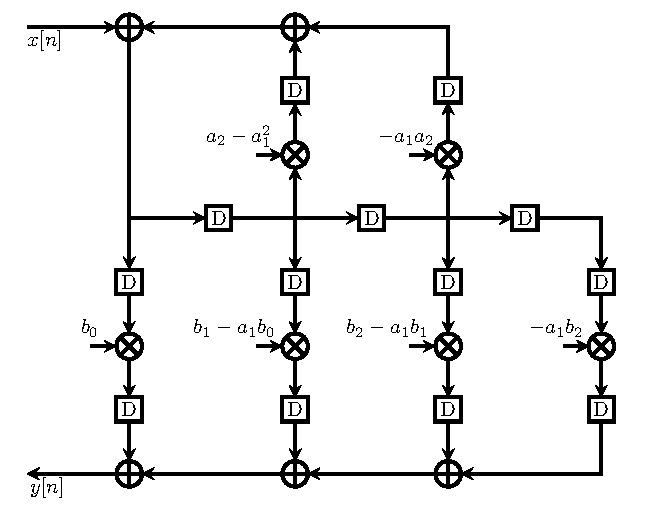
\includegraphics[width=.6\linewidth]{media/pipelined_lookahead_dfg.pdf}
	\caption{DFG of the filter}
	\label{fig:dfg}
\end{figure}
Figure \ref{fig:dfg} shows the DFG of the final architecture achieved at the end of the previous lab, by looking at which, one can quite positively state that the critical path is the delay of a single multiplier $T_m$, as it is almost certainly larger than the delay of three adders $3T_a$.
So one would expect the maximum frequency to remain constant as long as the multiplier used is the same and only the implementation of the adder is changed.

In fact, this is what happens in five cases out of six in table \ref{tab:fmax}: when using the carry-save based multiplier, the clock frequency is always limited by its delay, irrespective of the adder used. But when using the faster multiplier (\texttt{pparch}), the slowest ripple-carry adder seems to be the limiting factor, as the maximum frequency it allows is much lower than the one achieved with the same multiplier but faster adders.

So in this case the critical path seems to be the series of three adders, instead of the single multiplier. To verify this hypothesis, the DFG of the filter was slightly modified by introducing an additional pipeline stage to split the chain of $3$ adders into $2+1$ adders, as there is a feedforward cutset that allows it. By repeating the synthesis flow using the ripple-carry adder and the parallel prefix multiplier, the maximum frequency increased by around 10\%, from \SI{431.0}{\mega\hertz} to \SI{473.9}{\mega\hertz}. Even if this is not a 33\% improvement (probably due to design optimizations operated by the tool), as conceptually expected, it can nevertheless be concluded that the chain of three 24-bit ripple-carry adders was in the end the bottleneck of the design, being slower than one single 24-bit parallel prefix multiplier.

All in all, choosing the parallel-prefix multiplier combined with either carry-loohahead or parallel-prefix adders is the best option for speed: the maximum clock frequency is 60\% higher than the pair \texttt{pparch} multiplier/\texttt{rpl} adder, and 242\% faster than all carry-save multiplier based implementations.

\subsection{Cell area}
For what concerns area, table \ref{tab:area} shows that this figure seems to be once again mostly a matter of the type of multiplier chosen. Choosing the parallel-prefix multiplier is again the winning choice, as such implementations have a total area 38\% smaller than the one of designs based on a carry-save multiplier.

In the case of area, the choice of the type of adder does not seem to influence much the final figure, showing variations of less than 1\% among the three implementation, given the multiplier type.
\begin{table}[hbtp]
	\centering
	\begin{tabular}{clllll}
	\cline{1-5}
	\multicolumn{2}{|c|}{}                                                           & \multicolumn{3}{c|}{Adder}                                                                                                                                         &  \\ \cline{3-5}
	\multicolumn{2}{|c|}{\multirow{-2}{*}{Area [\si{\micro\meter^2}]}}                         & \multicolumn{1}{l|}{rpl}                             & \multicolumn{1}{l|}{cla}                             & \multicolumn{1}{l|}{pparch}                          &  \\ \cline{1-5}
	\multicolumn{1}{|c|}{}                             & \multicolumn{1}{l|}{csa}    & \multicolumn{1}{l|}{20987.4} & \multicolumn{1}{l|}{\cellcolor[HTML]{FFCCC9}21113.5} & \multicolumn{1}{l|}{20978.1} &  \\ \cline{2-5}
	\multicolumn{1}{|c|}{\multirow{-2}{*}{Multiplier}} & \multicolumn{1}{l|}{pparch} & \multicolumn{1}{l|}{15282.8} & \multicolumn{1}{l|}{15408.8} & \multicolumn{1}{l|}{\cellcolor[HTML]{9AFF99}15273.5} &  \\ \cline{1-5}
	\multicolumn{1}{l}{}                               &                             &                                                      &                                                      &                                                      &
	\end{tabular}
	\caption{Total area}
	\label{tab:area}
\end{table}

\subsection{Total power dissipation}
Power dissipation is clearly where the advantage of the parallel-prefix multiplier falls short. All implementations based on that show a 32-fold increase in dynamic power and a 14-fold increase in leakage power.

As always in digital design, as well as in life, one cannot get the best of both worlds, but has to settle for a trade-off, in this case between speed and power, as usual.
\begin{table}[hbtp]
	\centering
	\begin{tabular}{clllll}
	\cline{1-5}
	\multicolumn{2}{|c|}{\multirow{2}{*}{Power [\si{\micro\watt}]}} & \multicolumn{3}{c|}{Adder}                                                                                                                                                                                                     &  \\ \cline{3-5}
	\multicolumn{2}{|l|}{}                                                                                                        & \multicolumn{1}{l|}{rpl}                                                 & \multicolumn{1}{l|}{cla}                                                 & \multicolumn{1}{l|}{pparch}                                              &  \\ \cline{1-5}
	\multicolumn{1}{|c|}{\multirow{2}{*}{Multiplier}}                        & \multicolumn{1}{l|}{csa}                           & \multicolumn{1}{l|}{\begin{tabular}[c]{@{}l@{}}120.1\\ 3.1\end{tabular}} & \multicolumn{1}{l|}{\begin{tabular}[c]{@{}l@{}}120.1\\ 3.1\end{tabular}} & \multicolumn{1}{l|}{\begin{tabular}[c]{@{}l@{}}120.1\\ 3.1\end{tabular}} &  \\ \cline{2-5}
	\multicolumn{1}{|c|}{}                                                   & \multicolumn{1}{l|}{pparch}                        & \multicolumn{1}{l|}{\begin{tabular}[c]{@{}l@{}}3815\\ 43.5\end{tabular}} & \multicolumn{1}{l|}{\begin{tabular}[c]{@{}l@{}}3816\\ 43.5\end{tabular}} & \multicolumn{1}{l|}{\begin{tabular}[c]{@{}l@{}}3816\\ 43.5\end{tabular}} &  \\ \cline{1-5}
																			 &                                                    &                                                                          &                                                                          &                                                                          &
	\end{tabular}
	\caption{Dynamic and leakage power}
	\label{tab:pwr}
\end{table}

\subsection{Summing up}
If the main requirement is pure speed, then an architecture based on parallel-prefix Booth-recoded Wallace tree multipliers and carry-lookahead or parallel-prefix adders is the way to go.

If, on the other hand, the power budget is a limiting factor, one has to settle for lower processing speed and use CSA-based multipliers along with whichever adder they like best.

\section{MBE based Multiplier with Roorda's approach and Dadda Tree}
	Let's suppose to have a multiplication to be done between two numbers \textbf{x} and \textbf{y}.
	\begin{itemize}
		\item \textbf{x} is the multiplicand
		\item \textbf{y} is the multiplier
		\item $\bm{k_x}$ is the parallelism of \textbf{x}
		\item $\bm{k_x^{I}}$ is the number of bits representing the \textbf{I}nteger part of \textbf{x}
		\item $\bm{k_x^{F}}$ is the number of bits representing the \textbf{F}ractional part of \textbf{x}
		\item $\bm{k_y}$ is the parallelism of \textbf{y}
		\item $\bm{k_y^{I}}$ is the number of bits representing the \textbf{I}nteger part of \textbf{y}
		\item $\bm{k_y^{F}}$ is the number of bits representing the \textbf{F}ractional part of \textbf{y}
	\end{itemize}
	We want to perform the multiplication with the \textbf{MBE-radix4} encoded version of the multiplier \textbf{y}.
	This shrewdness allows us to reduce the number of partial products by half:
	indeed \textbf{y} is encoded with $\bm{k_y^{'}}$ symbols in $\{\pm{2}, \pm{1}, 0\}$. If $r=4$ is the radix:
	\begin{equation}
		\bm{k_y^{'} = \lceil \frac{k_y}{log_2(r)} \rceil = \lceil \frac{k_y}{2} \rceil}
	\end{equation}
	It's possible to MBE-encode a number in radix4 simply taking $\lceil \frac{k_y}{2} \rceil$ 1-bit overlapping triplets of it.
	If we consider \textbf{y} represented as a sequence of bits $\bm{y_{(k_y-1)} y_{(k_y-2)} \ldots
	y_{1} y_{0}}$ with the \textbf{LSB} in position \textbf{0}, then for correctly encoding \textbf{y} we must add
	a $\bm{y_{-1}}$ bit fixed at \textbf{0} to complete the first triplet. If $\bm{k_y}$ is odd then it will be
	added a bit $\bm{y_{k_y}}$ to complete also the last one.\\
	The encoded multiplier is then represented by the string of symbols
	\begin{equation}
		Y_{(\lceil \frac{k_y}{2} \rceil - 1)} Y_{(\lceil \frac{k_y}{2} \rceil - 2)} \ldots Y_{1} Y_{0}
	\end{equation}
	chosen from the set $\{\pm{2}, \pm{1}, 0\}$ wrt the table \ref{tab:mbe-tab}.

	\begin{table}[hbtp]
		\centering
		\begin{tabular}{|c|c|}
			\hline
			$y_{n+1} y_n y_{n-1}$ & $Y_{n}$  \\ \hline
			000 & 0  \\ \hline
			001 & 1  \\ \hline
			010 & 1  \\ \hline
			011 & 2  \\ \hline
			100 & -2 \\ \hline
			101 & -1 \\ \hline
			110 & -1 \\ \hline
			111 & 0  \\ \hline
		\end{tabular}
		\caption{MBE conversion table}
		\label{tab:mbe-tab}
	\end{table}

	The product is now between \textbf{x} and \textbf{Y}, the MBE-radix4 encoded version of \textbf{y}.
	Each partial product between a symbol of \textbf{Y} and \textbf{x} is performed using a multiplexer: two of
	the three bits which encode a symbol are used as control lines for the mux which can let pass either \textbf{0},
	or \textbf{x}, or \textbf{2x}. The other encoding bit is asserted only if the symbol is negative and it is used
	to complement the partial product. Moreover it will be added to the LSB of its partial product, to ensure a
	correct 2's complement negation. This way it's easy to obtain all the possible partial product: \textbf{0},
	\textbf{x}, \textbf{-x}, \textbf{-2x} and \textbf{2x}.
	It follows a figure (\ref{fig:v1-dp}) representing the DP of the multiplier.

	\begin{figure}[hbtp]
	\centering
	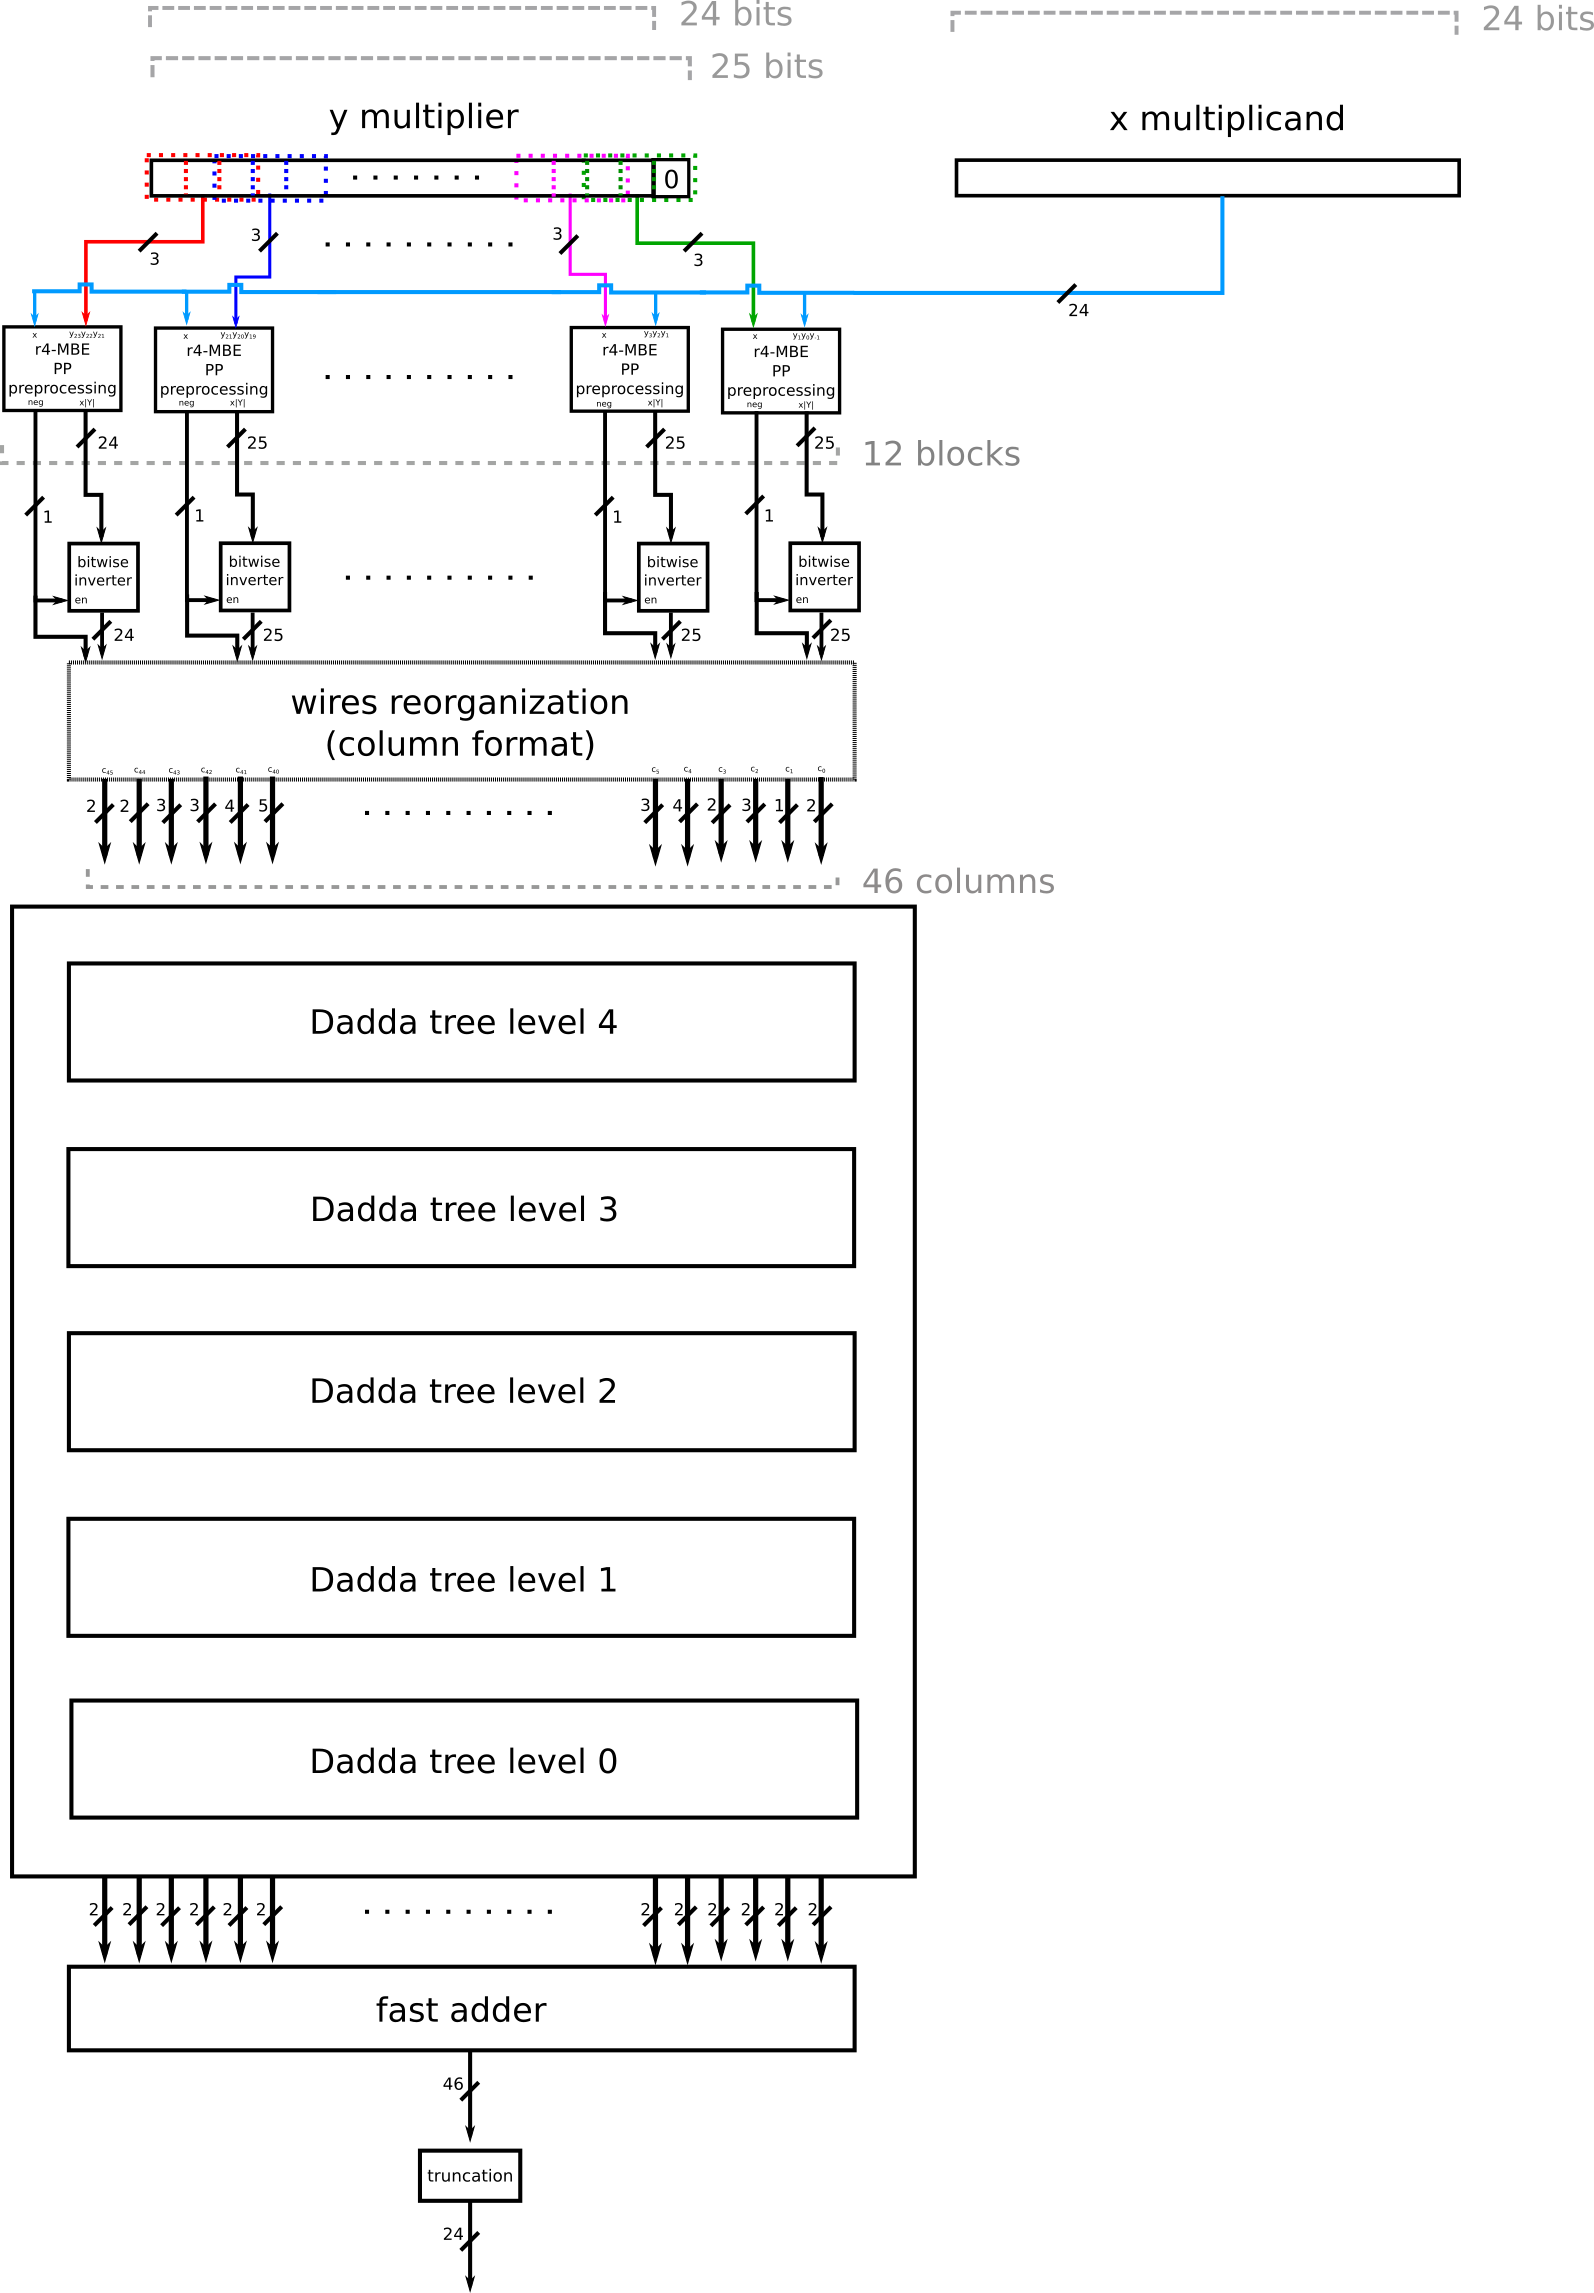
\includegraphics[width=.6\linewidth]{media/v1_abstract_DP.png}
	\caption{DP of the filter multiplier based on a DADDA tree, with Roorda's approach on MBE-r4 encoding}
	\label{fig:v1-dp}
	\end{figure}

	Since the entire operation has to last one clock cycle, all the partial products are obtained in parallel by $k^{'}_{y}$ encoding circuits and multiplexers. The derived tree is thought as a Dadda Tree and the number of FA is reduced
	simplifying the extended sign bits as proposed in \cite{roorda}.
	We have $\lceil \frac{k_y}{2} \rceil $ partial products to be compressed to only two terms with a Dadda Tree of FA/HA.
	Since with the multipliers in the filter we are not working with full dynamics, we can do not consider the first $\bm{k_y^I}$ MSBs, because they do not
	impact on the others. A saving in power and area is achieved this way. The number of integer bits of the lines of the filter was chosen not to let overflow occur anywhere in the filter; thus the number of integer bits is high enough and doesn't need to be increased. On the contrary the $\bm{k_y^F}$ LSBs are fundamental because of the carry of the sums in which they are involved, which can impact over the bits on their left. (More on this later)

	As Roorda highlighted, the bits of sign-extension can be thought as a series of \textbf{1} if the complement of the sign bit is added in its original position.
	This leads to a further optimization, because each column of \textbf{1}, starting from the rightmost one, can be simplified in advance noting that
	\begin{equation}
		\begin{cases}
        	?\ \ 1\\
        	?\ \ 1\\
        \end{cases}
        \implies
        \begin{cases}
        	?\ \ 0\\
        	?\ \ 0\\
        	1\
        \end{cases}
	\end{equation}
	and
	\begin{equation}
		\begin{cases}
        	?\ \ 1\\
        	?\ \ a\\
        \end{cases}
        \implies
        \begin{cases}
        	?\ \ \bar{a}\\
        	?\ \ 0\\
        	a\
        \end{cases}
	\end{equation}
	At the end we end up with the first row in which there is a string of "\textbf{10}", followed by a sequence of "$\bm{1\ \bar{p}_{k_{x}+1}^i}$" and then a triplet composed of "$\bm{\bar{p}_{k_{x}+1}^0 p_{k_{x}+1}^0 p_{k_{x}+1}^0}$". On the second row, under the first element $\bm{\bar{p}_{k_{x}+1}^0}$ of this triplet, there is $\bm{\bar{p}_{k_{x}+1}^1}$.\\
	\paragraph{Design of the multiplier} In our design we have
		\begin{itemize}
			\item $\bm{k_x = k_y = 24}$
			\item $\bm{k_x^{I} = k_y^{I} = 2}$
			\item $\bm{k_x^{F} = k_y^{I} = 22}$
			\item \textbf{12} partial products
			\item at most $\bm{\lceil \frac{k_y}{2} \rceil +1 = 13}$ elements in a single column
		\end{itemize}

	In a single column we can count up to 13 elements, because the MUX let only pass \textbf{x} multiplied for the absolute value of the symbol \textbf{Y}. Since this partial product passes only through a conditional negation block, to obtain a real C2 negation for a final partial product there is the need for a LSB to be summed. This "negative" bit (one of the three which encode a single symbol) is added
	to the LSB of its partial product: therefore we have 12+1 elements at most in a column (this can be seen in figure \ref{fig:v1-bind4}).
	This is not so bad, because with the Dadda Tree we are still in the case of having only 5 levels of adders (13 elements in a column at most).

	As said before, the sign extension bits can be reduced to chains of '1', and these chains can be "read" in column to be further simplified; the two MSB columns can be cut away because it's known that those columns will be only sign extension at the end of the multiplication. This is a reflection of what it was said before: in the filter architecture in which the multiplier is used the parallelism is $k = 24$ (Q2.22) for each words, but the coefficients are known and less than one\footnote{Be aware: this design is only valid under this assumption. Otherwise all the MSBs have to be taken into account.}, so the integer part of the product is always representable with 2 bits.

	The effect of this entire process is summarized in \ref{fig:v1-bind4}. The red dots are the "negative" bits to complete the C2 negation, white dots are the extended sign bits, each blue dot represent the negated sign bit of a partial product. The light blue dots are actually white ones, because they represent the extended sign bits of a partial product.

	The dashed red vertical line extrudes the two MSBs from the bindings of the adders.

	\begin{figure}[hbtp]
	\centering
	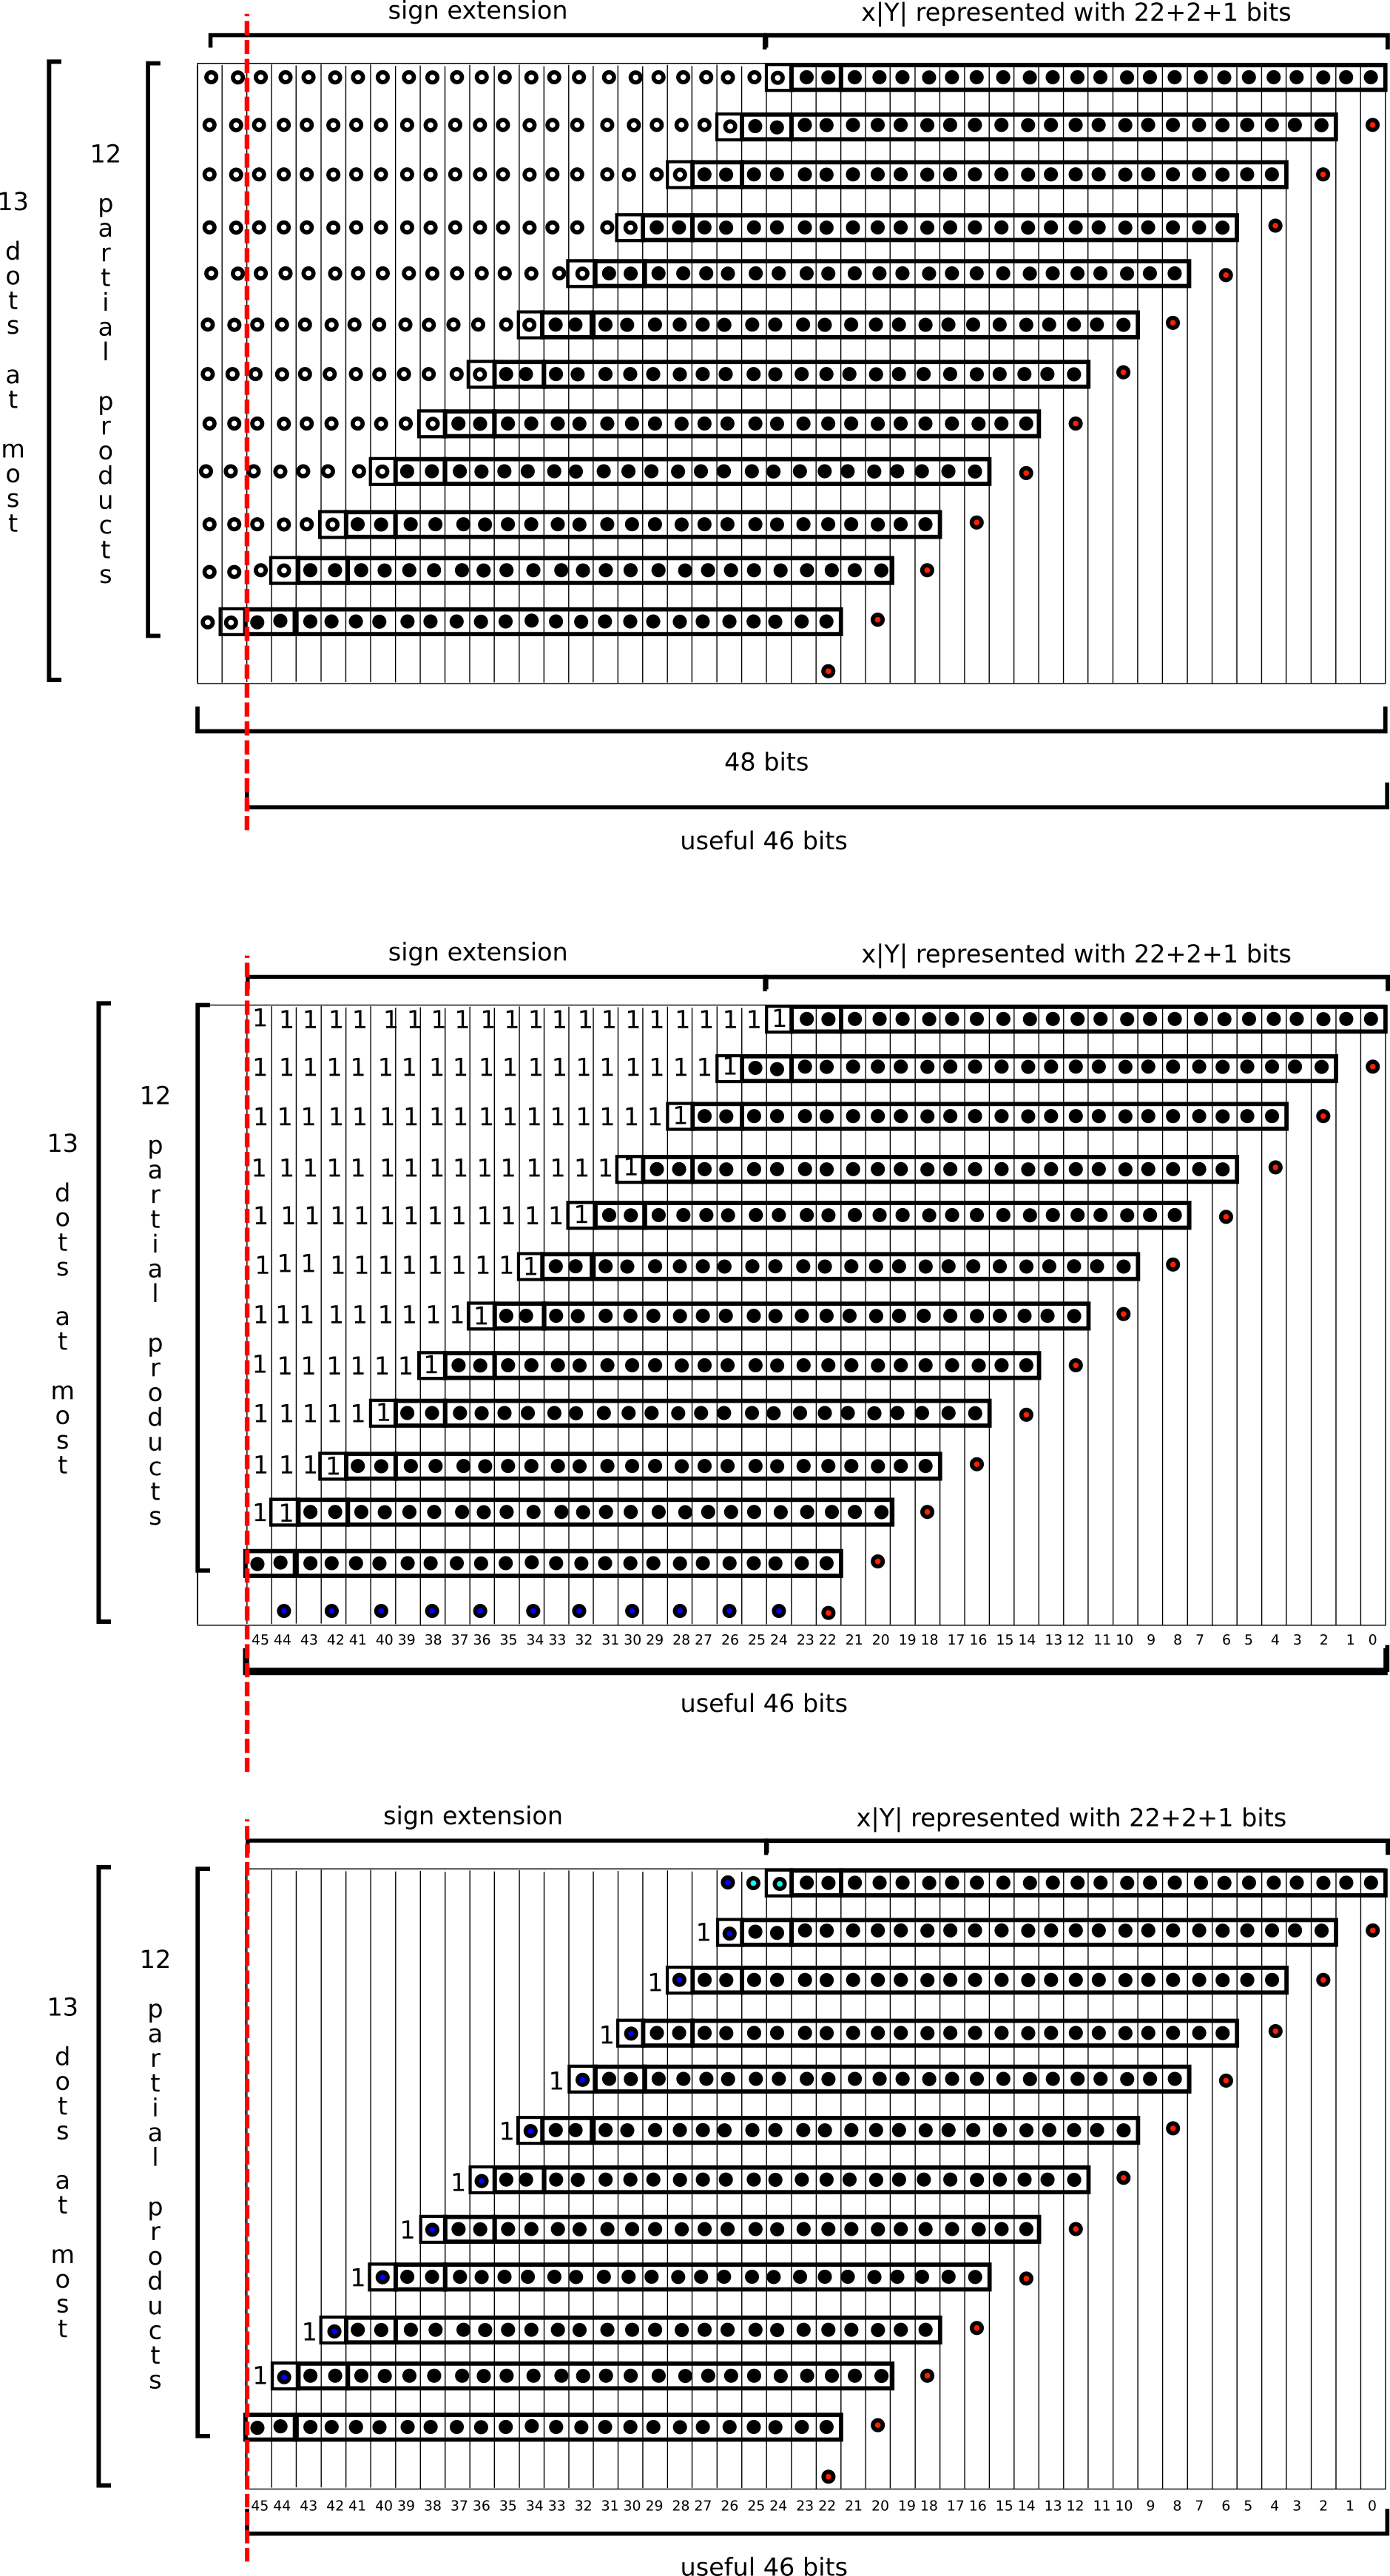
\includegraphics[width=.6\linewidth]{media/v1_FA_dadda_bindings_4.png}
	\caption{Applying the Roorda's method to reduce the numbers of adders}
	\label{fig:v1-bind4}
	\end{figure}

	For the first design the binding has been done by hand for each level of the tree. The following schematics show where FAs and HAs have been put.

	\begin{figure}[hbtp]
	\centering
	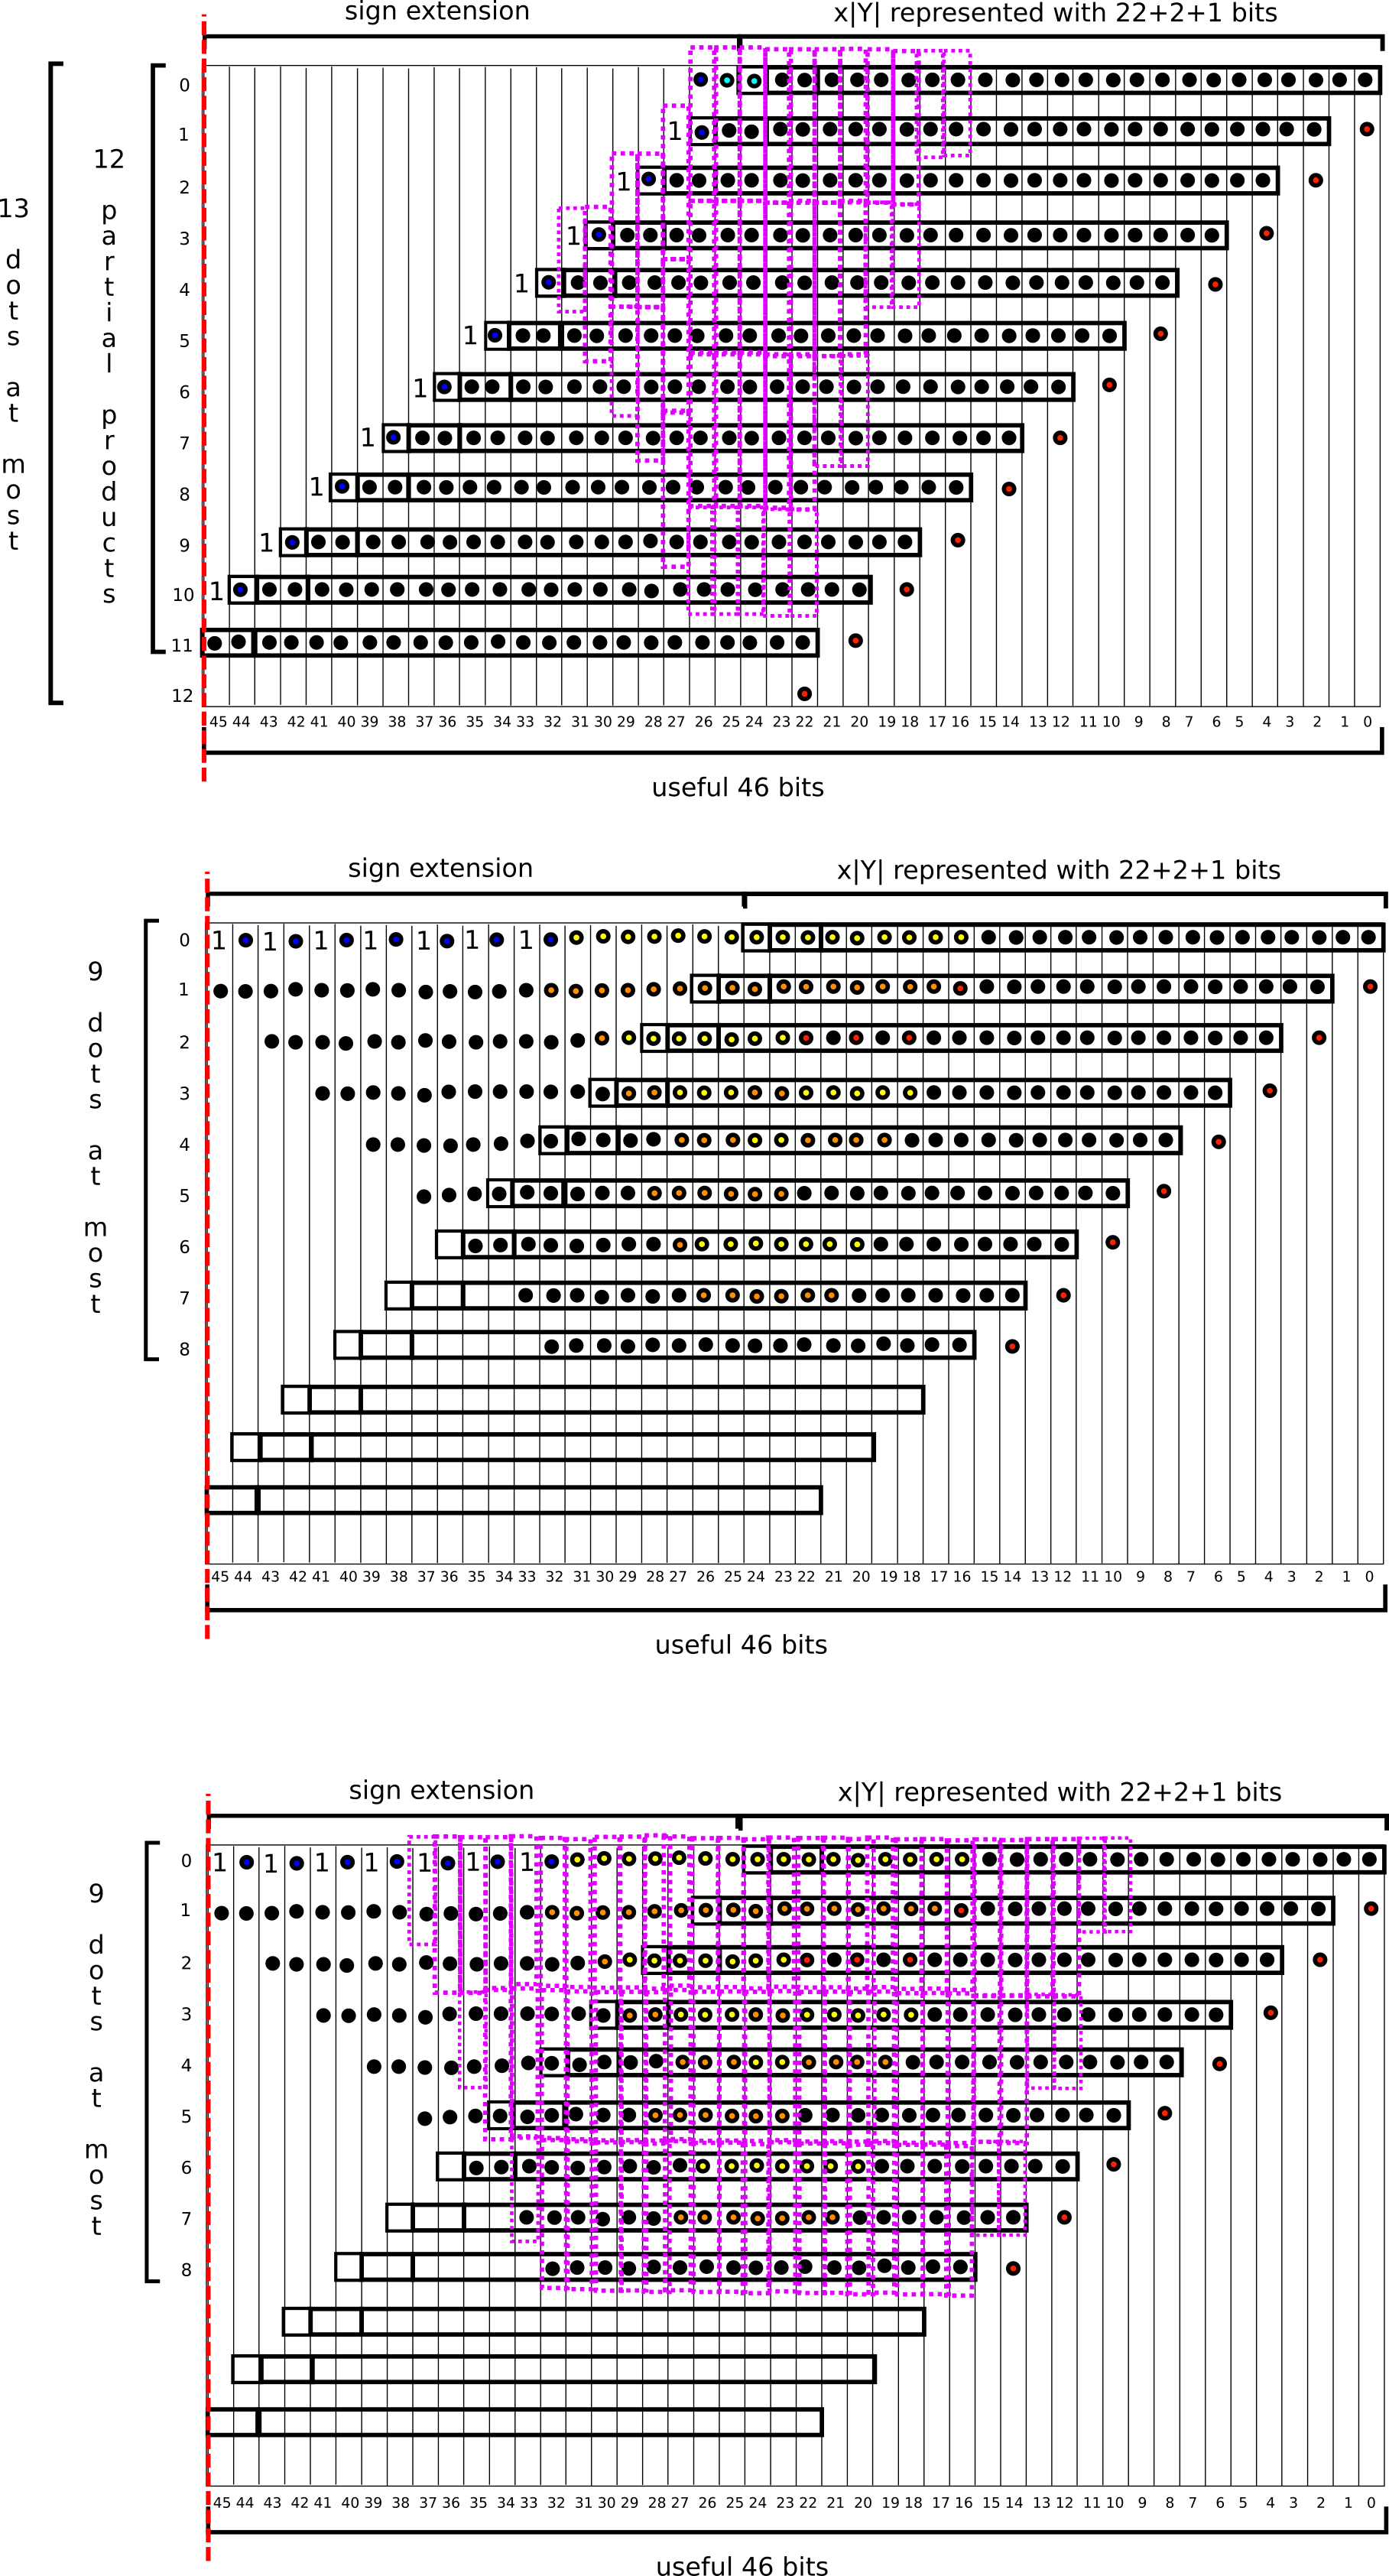
\includegraphics[width=.6\linewidth]{media/v1_FA_dadda_bindings_3.png}
	\caption{Applying the Roorda's method to reduce the numbers of adders}
	\label{fig:v1-bind3}
	\end{figure}

	\begin{figure}[hbtp]
	\centering
	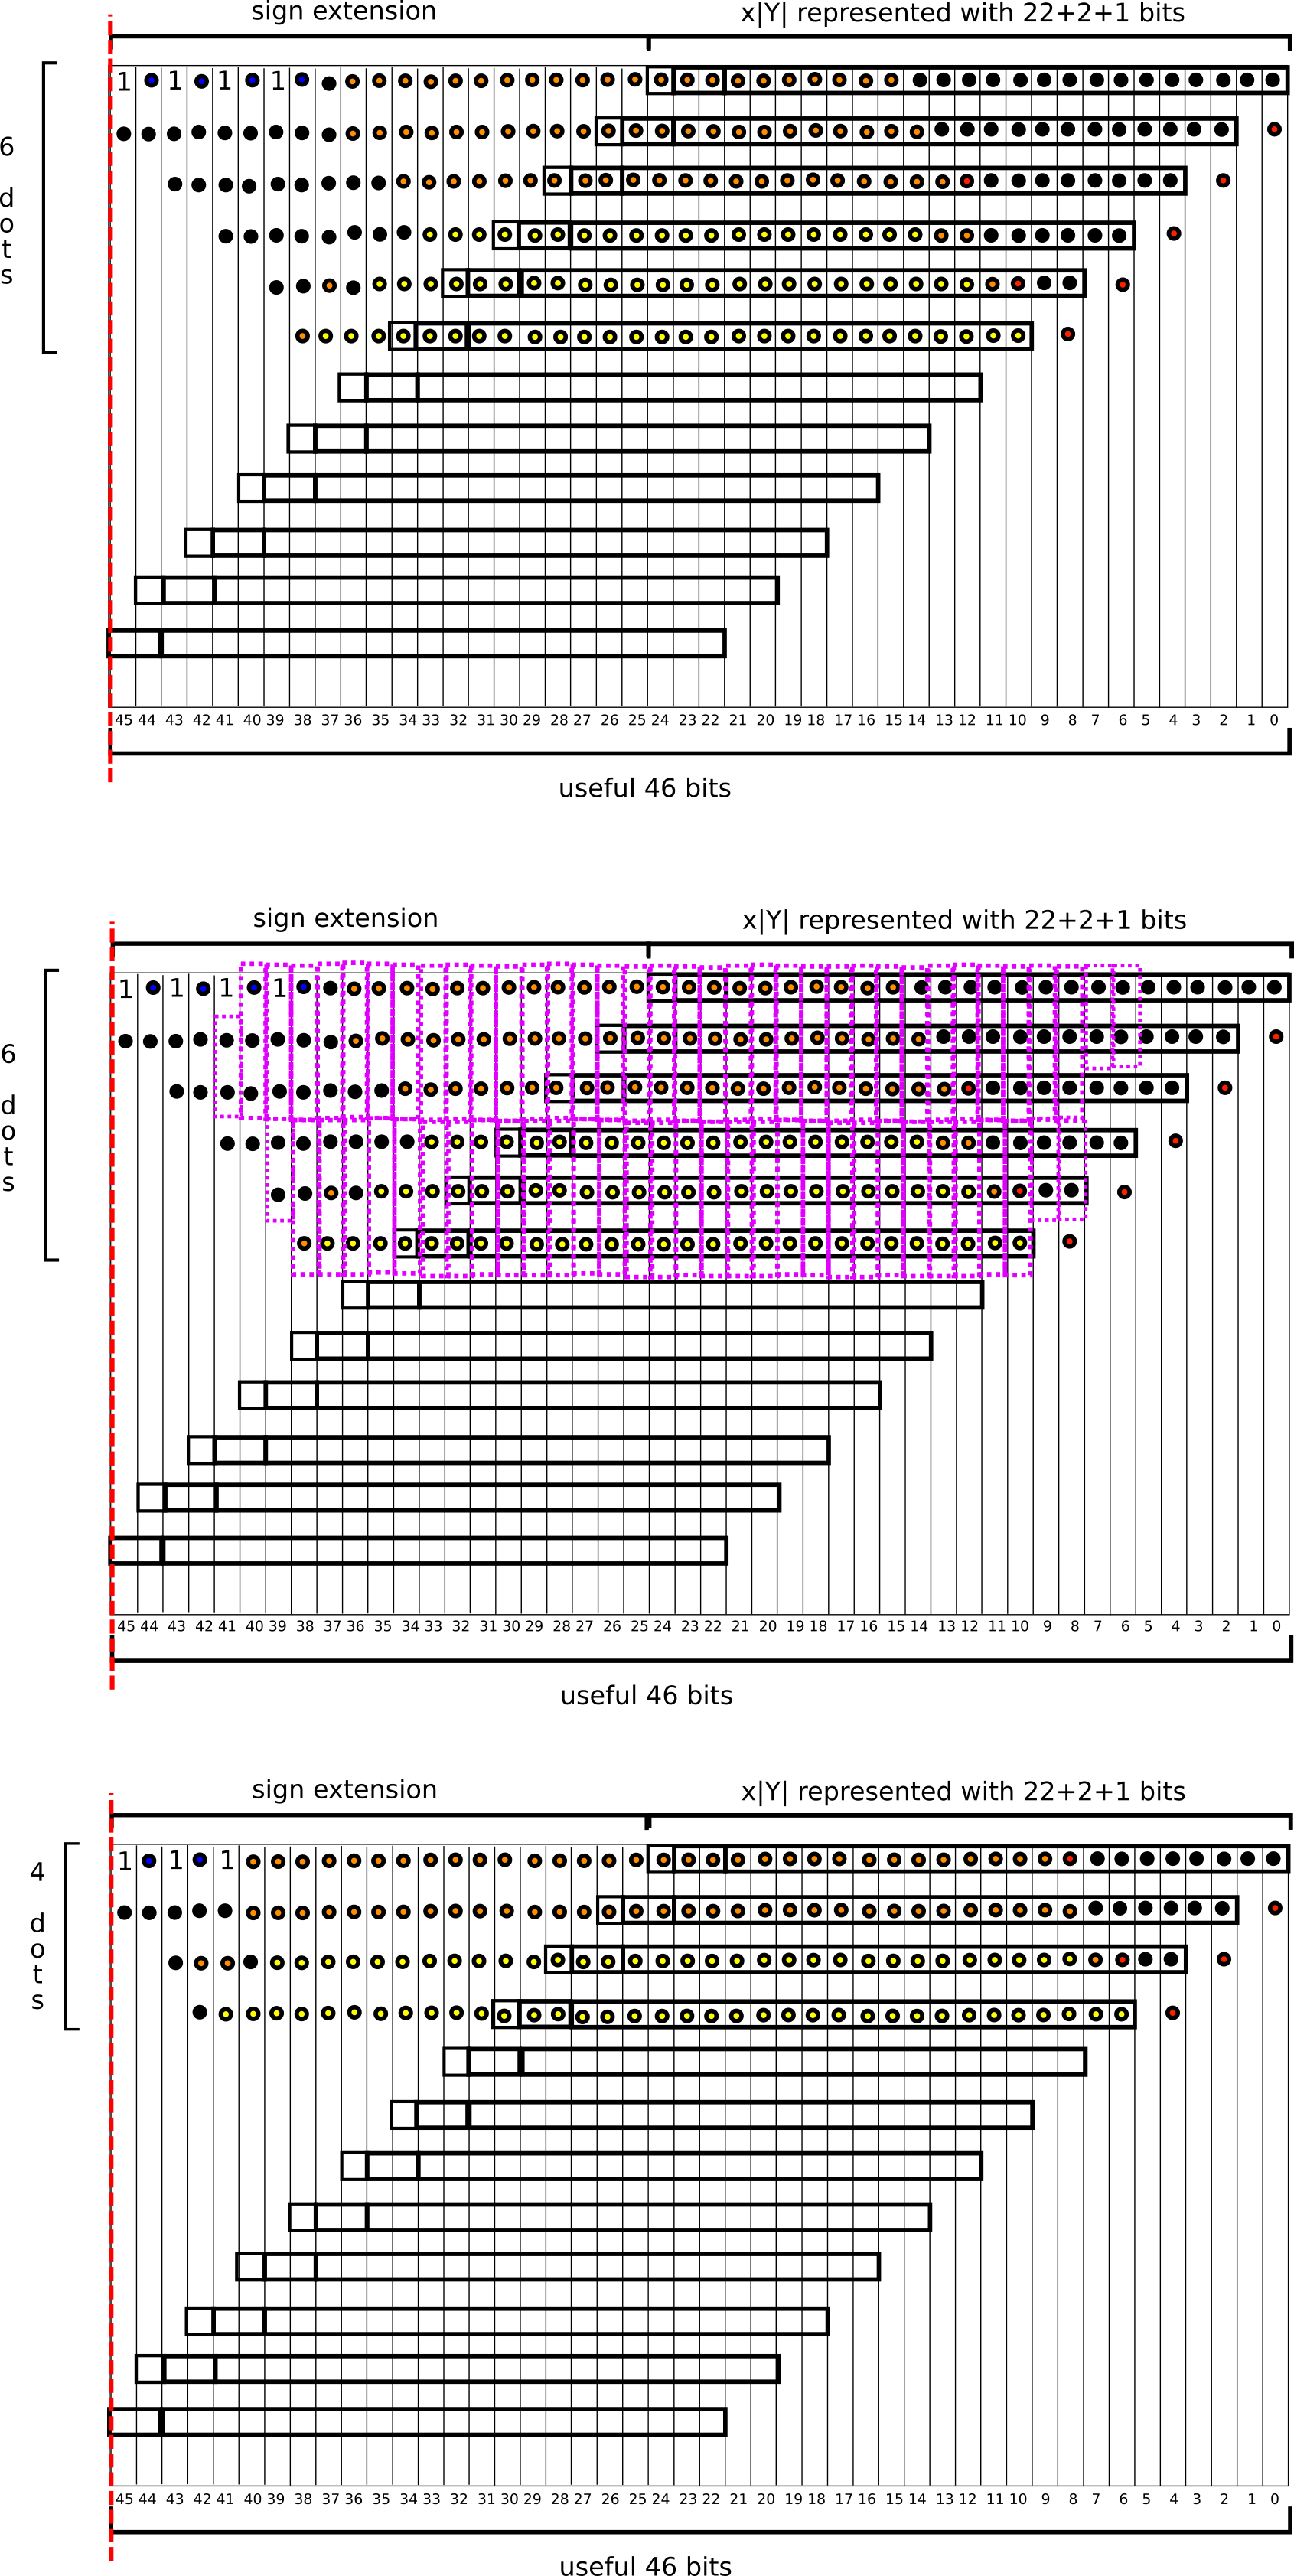
\includegraphics[width=.6\linewidth]{media/v1_FA_dadda_bindings_2.png}
	\caption{Applying the Roorda's method to reduce the numbers of adders}
	\label{fig:v1-bind2}
	\end{figure}

	\begin{figure}[hbtp]
	\centering
	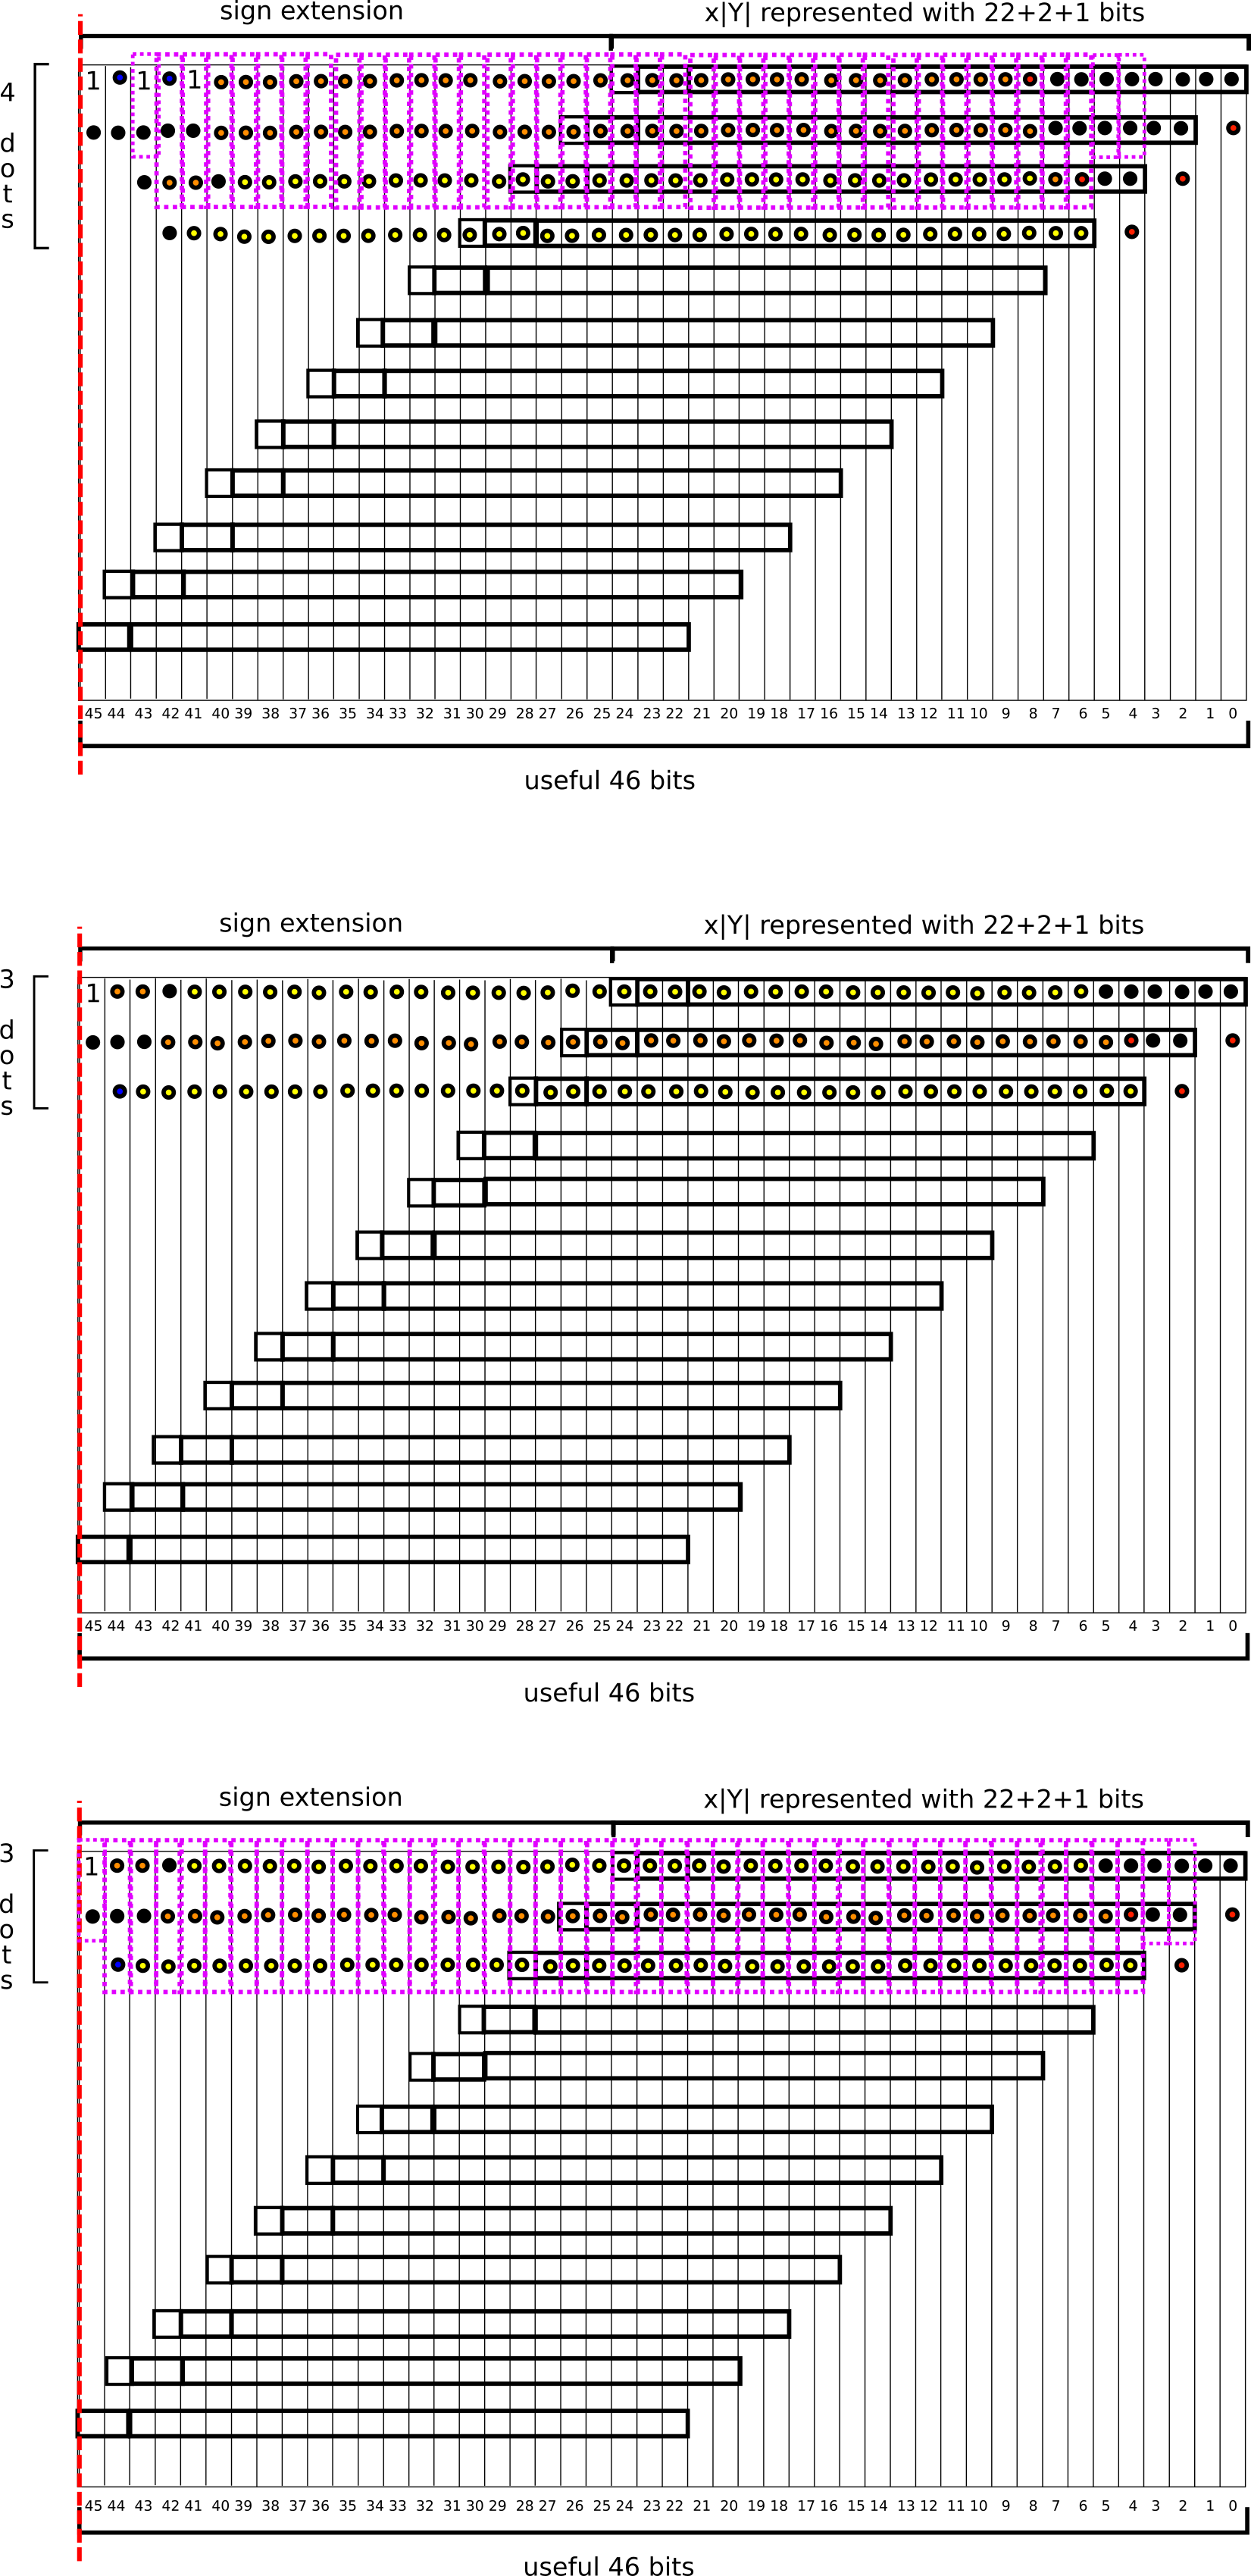
\includegraphics[width=.6\linewidth]{media/v1_FA_dadda_bindings_1.png}
	\caption{Applying the Roorda's method to reduce the numbers of adders}
	\label{fig:v1-bind1}
	\end{figure}

	\begin{figure}[hbtp]
	\centering
	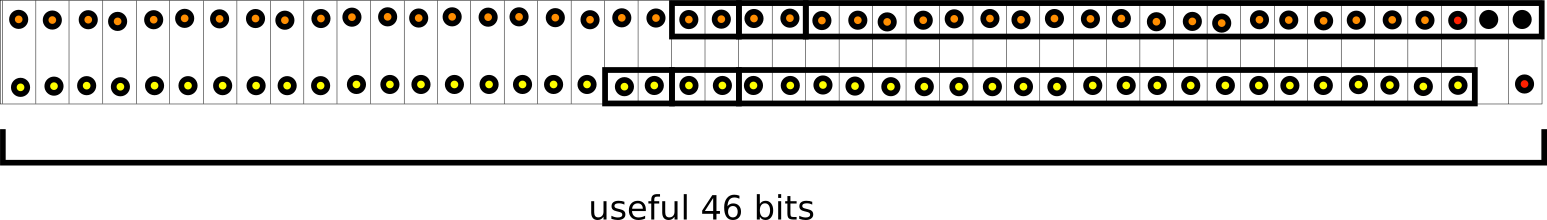
\includegraphics[width=.6\linewidth]{media/v1_FA_dadda_bindings_0.png}
	\caption{Applying the Roorda's method to reduce the numbers of adders}
	\label{fig:v1-bind0}
	\end{figure}

	The last operation in an addition, and can be implemented by a fast adder. In our design the adder has been kept behavioural, because the main aim of this work is to study a multiplier and how the uncertainty of the results changes with the adoption of some tricks to improve the figures of merit without keeping full precision.

	\paragraph{VHDL description} A new method to write VHDL has been adopted to speed up the description of the circuit. The first part (common to all design) in which the partial product are computed was described by hand, but the part of the Dadda trees and the bindings are written by a parametric python script. This allows a great re-usability and a fast method to compare multiple instances with different styles of binding.
	Furthermore this way of working is not prone to errors, because the number of lines of hand written code is drastically reduced.
	Another advantage of the script is that the VHDL description can scale up well with the number of bits.

	The strategy to write the VHDL is the following: for each DADDA level a matrix of $std\_logic\_vector$ is created. From one level to the next only the useful bits are assigned or processed (all the assignments are bitwise assignments from one matrix to the next).

	Adders are instantiated where they are needed, and the port map follows the same "one matrix to the next" strategy used for the assignments.

	To implement this design the first hand written part of the file prepares the first matrix (in the following it will be used the term "grid") called \textbf{grid5}

	At first the partial product are assigned to the matrix cells with standard logic vector assignments, to reproduce the first scheme of \ref{fig:v1-bind4}. Then all the dots are flattened to the top of the grid \textbf{before} the first binding. This is in contrast with the scheme of \ref{fig:v1-bind3}, where the first bininding is done before the flattening.
	All the other figures show exactly what is described by the VHDL.

	The process of bringing all the bits to the ceiling of the grid is done by the hand written part of the file and it is word length dependent. It's not difficult to implement it in the python script, and this improvement would make the entire multiplier parametric.

	\subparagraph{The python script}

	As already said only the first part of the VHDL has been kept hand written. The dadda-bindings of the tree, the instantiation of the adders and the assignments from one grid to the next are fully automatic.

	In its basic version it needs only a list with a number of cells equal to the number of columns of the grid, with each cell containing the number of elements of the corresponding column. With this information the script, starting from the rightmost column (i.e. from the column of the LSB of the result), analyzes if there's the need for a compressor (a FA, HA or an approximated one) and writes into another list the number of adders needed.

	Then the main routine writes on the file all the component instantiations and the assignments to end up with a new grid with all the elements flattened to its top, respecting the DADDA strategy to have the minimum number of levels with an ALAP resources binding approach.

	Both for bindings and assignments the script has to deal with the carries of the compressors, to work well. The details of the routine can be found looking at the code.

	The script works also for versions 2 and 3 of the project: it receives parameters to design a multiplier in which an arbitrary number of LSB columns does not appear in the tree (version2 of the project) and to use a variable number of approximated compressors when the binding is performed (version 3 of the project). These two design choices can be important to save area and power (and maybe to increase the clock frequency, but it depends on the used ports and on the technology).
	A more detailed description of the working principles of the script in designing v2 and v3 multipliers can be found in the corresponding sections.

	The script produces also a drawing of each level of the tree: this output can be redirected on the prompt or to a file and used to check the correctness of the result of the bindings when a VHDL is automatically written (figures \ref{fig:dadda_terminal0}, \ref{fig:dadda_terminal1}, \ref{fig:dadda_terminal2}, \ref{fig:dadda_terminal3}).

	\begin{figure}[hbtp]
	\centering
	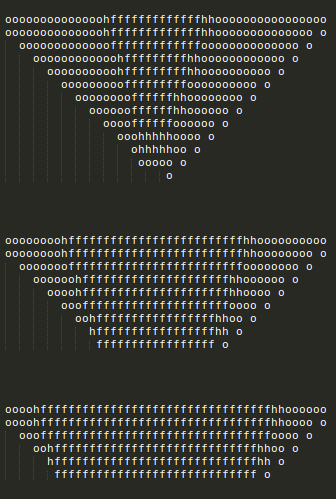
\includegraphics[width=0.5\linewidth]{media/dadda0.png}
	\caption{Dadda terminal drawing (0), compression level: 0\%}
	\label{fig:dadda_terminal0}
	\end{figure}

	\begin{figure}[hbtp]
	\centering
	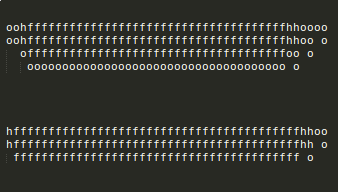
\includegraphics[width=0.5\linewidth]{media/dadda1.png}
	\caption{Dadda terminal drawing (1), compression level: 0\%}
	\label{fig:dadda_terminal1}
	\end{figure}

	\begin{figure}[hbtp]
	\centering
	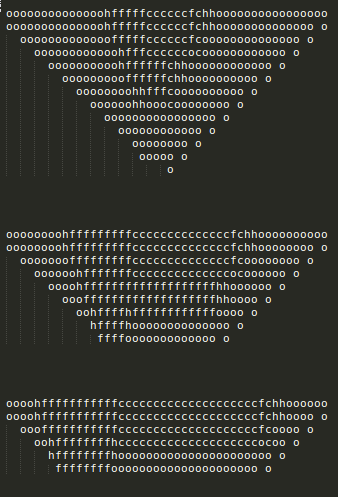
\includegraphics[width=0.5\linewidth]{media/dadda2.png}
	\caption{Dadda terminal drawing (0), compression level: 70\%}
	\label{fig:dadda_terminal2}
	\end{figure}

	\begin{figure}[hbtp]
	\centering
	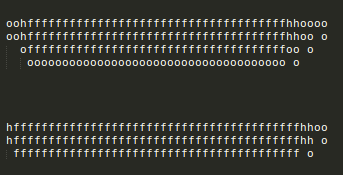
\includegraphics[width=0.5\linewidth]{media/dadda3.png}
	\caption{Dadda terminal drawing (1), compression level: 70\%}
	\label{fig:dadda_terminal3}
	\end{figure}

	\section{Approximated architectures analysis}
	\subsection{Approximated multiplier architecture}
	The main idea for \textit{version 2}, as suggested in the lab paper, is to approximate the partial products in order to gain mainly in terms of power and area.
	This can be achieved by simply truncating \textbf{k} leftmost bits of every partial product before allocating any half or full adder in those positions, as shown in the following picture.
	Obviously we pay in precision since we loose the contribution on final resut for those bits we've set to '0'. In the following sections we will explain the analysis on how multiplier and filter characteristics changes by varying the k paramiter.


	\subsection{Approximations with 4-2 compressors}
	A further approach, to improve the three figures of merit of the design, is to substitute the FAs and the HAs with approximated compressors which take in input four bits with the same weight and give in output one bit of the same weight of the inputs and one bit with double this weight.
	In \ref{yin} this technique with a cutting of the LSBs was adopted, and it was shown good results wrt the main figures of merit.

	The approximation is variable and it is function of how many 4-2 compressors are used in the multiplier tree and where. The proposed compressor implementation can only miss the sum bit, while the carry one is always correct.
	This implies that the maximum error is related to the weight of the column in which the compressor has been allocated: it's easy to understand that a approximated compressors allocated on the \textit{left} bits create an error higher than the one produced by compressors put more on the right.

	The script we used for the standard version allows also to generate many multipliers with a different number of approximated compressors, allocated in different positions.

	\paragraph{script} The basic version of the script performs the binding only with FAs and HAs. It starts from the LSB and assigns as many FAs as possible where needed to compress the bits' number of a certain column following DADDA's approach. If the reduction from one level to the next is possible using an HA instead of the last FA, then an HA is assigned.

	To create an approximated multiplier the binding is performed giving precedence to the 4-2 compressor instead of the FA. Ideally a complete covering with 4-2 compressors can be done, but in order to analyze and fully understand how system-level characteristics change with the number of approximated compressors in the architecture, the possibility to give as an argument a percentage of approximated adders to be inserted in the binding was introduced in the script.
	Indeed it is possible to ask for a multiplier with a compression level of $40\ \%$, and this means that only the $40\ \%$ of the compressors will be put, starting from the MSB or LSB. This last choice is determined by the other passed parameter, the "startingDirection" one. So, the algorithm calculates how many compressors would be put if the copression level was 100\%, then it inserts only the asked percentage of them.

	Where a compression is needed but no compressors can be put, FAs and HAs are used instead. The latters are used also to respect the DADDA "maximum rows" allowed in the tree levels : the algorithm looks always for the minimum compression which allows the minimum number of levels.

	\subsection{Data collection}
	In order to understand better how we solved the data collection part, for the explanation we will consider the following flow chart.
	\begin{figure}[hbtp]
	\centering
	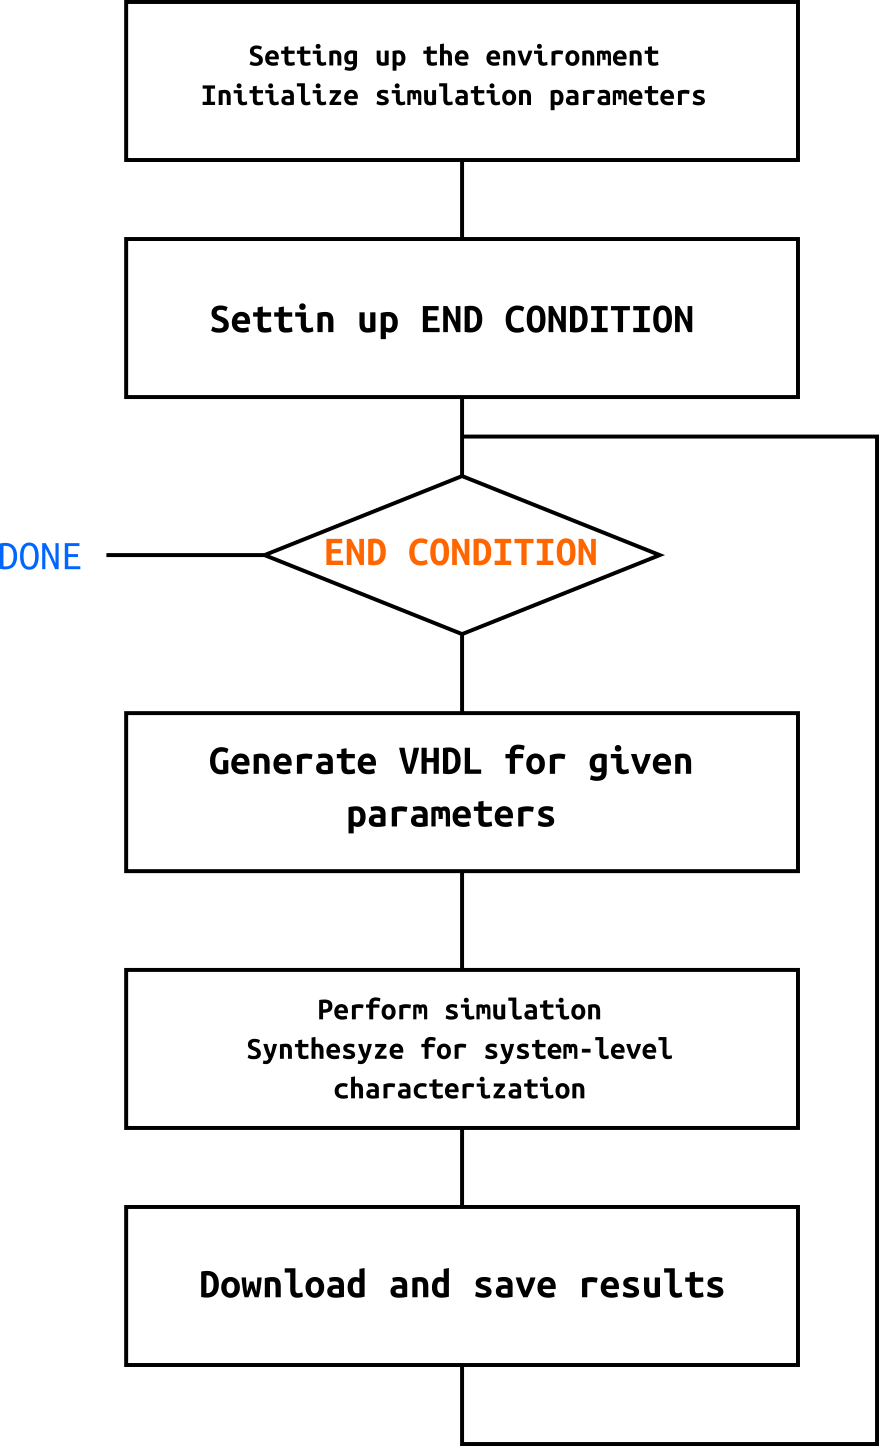
\includegraphics[width=0.5\linewidth]{media/Algorithm_Flowchart.png}
	\caption{Data collection algorithm}
	\label{fig:v1-bind0}
	\end{figure}

	A Python script performs all these actions calling subfuntions already used for first lab and others done ad-hoc for this step.
	\paragraph{Setting the environment} The first passage consists of connecting to the server and cleaning working directories locally and remotely. Then input sample vectors are generated and uploaded to the server with the specific scripts and all the common files needed for simulation. In this first step, model of the IIR filter and of a multiplier are run to produce correct results, useful for the final analysis.

	\paragraph{End condition} The \textit{END CONDITION} is set according on which type of data we want to collect. Examples can be:
	\begin{itemize}
		\item for Number\_of\_LSB\_to\_drop in renge(0,10,1)
		\item for Persantege\_of\_approx\_compressor in range(0,50,5)
	\end{itemize}
	In the first case we are cycling from 0 to 9, incrementing the iterator by one each cycle. Similar is the second case.\newline
	In this way we can obtain all the data we need launching just once the script.

	\paragraph{Generate VHDL} First step of the loop is the automatic generation of the VHDL description of the Dadda multiplier. To execute the generator we have to specify three parameters:
	\begin{itemize}
		\item Compression Level, percentage of approximated compressor
		\item Starting Direction, left or right
		\item Aproximation Bits, number of leftmost bits that have to be truncated
	\end{itemize}
	Notice that it is possible to generate a hybrid multiplier whith \textit{k} bits truncated and a certain \textit{h\%} of 4-to-2 compressor.

	\paragraph{Simulation and Synthesis} The simulation and synthesis part is performed twice: once just for the multiplier, and the second time for the whole filter. This is done to understand how different "types" of multiplier impact on the multiplication itself and to the final result of the filter. From the input parameters we gave at the previous step to the final output we can keep track of all the dataflow through our aproximated block.

	We have to notice that it is possible to set a flag to enable the Compile Ultra option of Synopsis. This will couse the elaboration time to increase but a more precise synthesis of the circuit.

	\paragraph{Result downlaod} Last step consist of saving locally results and report from previous elaboration.

	\subsection{Data Analysis}
	Starting from all the files downloaded after simulation and synthesis a third script computes error statistics from approximated-architecture outputs and collects significant values from synthesis reports.
	Actual list of action performed is the following one:

	\begin{itemize}
		\item Test the results from truncated architecture multiplier with Python model.
		\item Compute error statistics from truncated multiplier.
		\item Compute error statistics from filter with truncated multiplier.
		\item Collect synthesis results from truncated multiplier
		\item Collect synthesis results from filter with truncated multiplier.
    \item Compute error statistics from multiplier with approx. compressors.
    \item Compute error statistics from filter with multiplier with approx. compressors.
   	\item Collect synthesis results from multiplier with approx. compressors.
    \item Collect synthesis results from filter with multiplier with approx. compressors.
	\end{itemize}

	\paragraph{Error statistics computation} A fast but important review has to be done in order to understand how the error analysis is handled.
	We decided to use both absolute and relative distance between exact result and approximate one, since is the only way to have an idea of how much approximation parameters influence final result. The relative distance is calculated as:
	\begin{equation}
		e_{i}=\frac{Se_{i}-Sa_{i}}{Se_{i}}
	\end{equation}
	All the results processed by a given architecture are analysed keeping track of the \textbf{maximum and the average relative error}. All these values are then stored into log files ready to be used to create graphs or do any kind of analysis.\\
	For the simulation we decided to generate 250000 couples of inputs for the multiplier and 250000 samples for the filter. The simulation was performed on the VHDL/Verilog model before the synthesis. 

	\subsection{Multiplier with compressors}

	An useful metric to evaluate an approximated multiplier is the \textbf{NMED}. This parameter assumes a mean over the errors of all the outputs relative to all the inputs. This is a huge task when we have to deal with high parallelisms. So we used a high set of inputs and calculated the mean and maximum error. Calculating the NMED would be an improvement for our work.

	\paragraph*{Simulation} Ten multipliers have been tested besides the original, each of them with a different percentage of inexact compressors among the correct ones. The relative and absolute error are reported in the following tables and plots. 

	\begin{table}[hbtp]
		\centering
		\begin{tabular}{|c|c|c|c|c|}
		\hline
		\textbf{\begin{tabular}[c]{@{}c@{}}Multiplier\\ compression level\end{tabular}} & \textit{\textbf{\begin{tabular}[c]{@{}c		@{}}Max error\\ {[}LSB{]}\end{tabular}}} & \textit{\textbf{\begin{tabular}[c]{@{}c@{}}Avg. error\\ {[}LSB{]}\end{tabular}		}} & \textit{\textbf{Max relative error}} & \textit{\textbf{Avg. relative error}} \\ \hline
		\textbf{10\%}                                                                   & 		1.0                                                                             & 		-0.012                                                                           & -4.85e-05                            &		 -7.20e-08                             \\ \hline
		\textbf{20\%}                                                                   & 		1.0                                                                             & 		-0.071                                                                           & 1.1e-03                              &		 8.80e-07                              \\ \hline
		\textbf{30\%}                                                                   & 		-3.0                                                                            & 		-0.239                                                                           & -2.1e-02                             &		 -2.12e-05                             \\ \hline
		\textbf{40\%}                                                                   & 		-7.0                                                                            & 		-1.016                                                                           & 1.2e-03                              &		 -2.51e-06                             \\ \hline
		\textbf{50\%}                                                                   & 		-18.0                                                                           & 		-4.754                                                                           & -2.1e-01                             &		 -2.300e-04                            \\ \hline
		\textbf{60\%}                                                                   & 		-75.0                                                                           & 		-28.254                                                                          & -6.38e-01                            &		 -7.4e-04                              \\ \hline
		\textbf{70\%}                                                                   & 		16777090.0                                                                      & 		16646.29                                                                         & 356959.36                            &		 356.95                                \\ \hline
		\textbf{80\%}                                                                   & 		16776178.0                                                                      & 		32447.17                                                                         & 356939.95                            &		 376.83                                \\ \hline
		\textbf{90\%}                                                                   & 		16774518.0                                                                      & 		77205.154                                                                        & 356667.61                            &		 387.53                                \\ \hline
		\textbf{100\%}                                                                  & 		16773938.0                                                                      & 		3354.786                                                                         & 356892.30                            &		 366.37                                \\ \hline
		\end{tabular}
		\caption{Multiplier, simulation and error results}
		\label{tab:mult_sim}
	\end{table}

	\paragraph*{Synthesis} All the multipliers were synthesized and informations of area and timing reported. The minimum delay was found in theoretical way asking Design Compiler to reach a null arrival time.

	\begin{table}[hbtp]
		\centering
		\begin{tabular}{|c|c|c|c|}
		\hline
		\textbf{\begin{tabular}[c]{@{}c@{}}Multiplier\\ compression level\end{tabular}} & \textit{\textbf{\begin{tabular}[c]{@{}c		@{}}Area\\ {[}$um^2${]}\end{tabular}}} & \textit{\textbf{\begin{tabular}[c]{@{}c@{}}Delay\\ {[}ns{]}\end{tabular}}} & \		textit{\textbf{\begin{tabular}[c]{@{}c@{}}Max. frequency\\ {[}MHz{]}\end{tabular}}} \\ \hline
		\textbf{0\%}                                                                    & 		3801                                                                       & 		1.39                                                                       & 		719                                                                                  \\ \hline
		\textbf{10\%}                                                                   & 		3744                                                                       & 		1.39                                                                       & 		719                                                                                  \\ \hline
		\textbf{20\%}                                                                   & 		3947                                                                       & 		1.35                                                                       & 		740                                                                                  \\ \hline
		\textbf{30\%}                                                                   & 		3803                                                                       & 		1.35                                                                       & 		740                                                                                  \\ \hline
		\textbf{40\%}                                                                   & 		3453                                                                       & 		1.35                                                                       & 		740                                                                                  \\ \hline
		\textbf{50\%}                                                                   & 		3164                                                                       & 		1.38                                                                       & 		724                                                                                  \\ \hline
		\textbf{60\%}                                                                   & 		3670                                                                       & 		1.30                                                                       & 		769                                                                                  \\ \hline
		\textbf{70\%}                                                                   & 		3270                                                                       & 		1.29                                                                       & 		775                                                                                  \\ \hline
		\textbf{80\%}                                                                   & 		3164                                                                       & 		1.28                                                                       & 		781                                                                                  \\ \hline
		\textbf{90\%}                                                                   & 		2971                                                                       & 		1.28                                                                       & 		781                                                                                  \\ \hline
		\textbf{100\%}                                                                  & 		2829                                                                       & 		1.31                                                                       & 		763                                                                                  \\ \hline
		\end{tabular}
		\caption{Multiplier, area and timing synthesis reports}
		\label{tab:mult_syn}
	\end{table}

	\subsection{IIR filter}
	For each multiplier, a filter was tested and then synthesized.

	\paragraph*{Simulation} As it has already been said, 250000 samples was given in input to the filter with the multipliers. It follows the results.  

	\begin{table}[hbtp]
		\centering
		\begin{tabular}{|c|c|c|c|c|}
		\hline
		\textbf{\begin{tabular}[c]{@{}c@{}}IIR filter\\ compression level\end{tabular}} & \textit{\textbf{\begin{tabular}[c]{@{}c		@{}}Max error\\ {[}LSB{]}\end{tabular}}} & \textit{\textbf{\begin{tabular}[c]{@{}c@{}}Avg. error\\ {[}LSB{]}\end{tabular}		}} & \textit{\textbf{Max relative error}} & \textit{\textbf{Avg. relative error}} \\ \hline
		\textbf{10\%}                                                                   & 		0                                                                               & 		0                                                                                & 0                                    &		 0                                     \\ \hline
		\textbf{20\%}                                                                   & 		0                                                                               & 		0                                                                                & 0                                    &		 0                                     \\ \hline
		\textbf{30\%}                                                                   & 		0                                                                               & 		0                                                                                & 0                                    &		 0                                     \\ \hline
		\textbf{40\%}                                                                   & 		1                                                                               & 		0.001                                                                            & 7.79e-04                             &		 7.78e-07                              \\ \hline
		\textbf{50\%}                                                                   & 		-1                                                                              & 		-0.005                                                                           & 5.08e-03                             &		 -6.40e-06                             \\ \hline
		\textbf{60\%}                                                                   & 		-1                                                                              & 		-0.014                                                                           & 2.22e-02                             &		 -3.48e-05                             \\ \hline
		\textbf{70\%}                                                                   & 		-1                                                                              & 		-0.086                                                                           & 1.42e-01                             &		 2.70e-04                              \\ \hline
		\textbf{80\%}                                                                   & 		-4                                                                              & 		-1.093                                                                           & -1                                   &		 3.87e-03                              \\ \hline
		\textbf{90\%}                                                                   & 		8183.0                                                                          & 		15.44                                                                            & 8177.0                               &		 10.95                                 \\ \hline
		\textbf{100\%}                                                                  & 		-8177.0                                                                         & 		2.84                                                                             & 371.04                               &		 0.63                                  \\ \hline
		\end{tabular}
		\caption{IIR filter, simulation and error results}
		\label{tab:iir_sim}
	\end{table}

	\paragraph*{Synthesis} The results of the synthesis are visible in the following table and figure. The synthesis was done letting the program to perform retiming, this is why the delay is lower than for a single multiplier. These results were found without giving the \textit{compile\_ultra} command, only to have an idea of the trend.

	\begin{table}[hbtp]	
		\centering
		\begin{tabular}{|c|c|c|c|}
		\hline
		\textbf{\begin{tabular}[c]{@{}c@{}}IIR filter\\ compression level\end{tabular}} & \textit{\textbf{\begin{tabular}[c]{	@{}c	@{}}Area\\ {[}$um^2${]}\end{tabular}}} & \textit{\textbf{\begin{tabular}[c]{@{}c@{}}Delay\\ {[}ns{]}\end{tabular}	}} & \	textit{\textbf{\begin{tabular}[c]{@{}c@{}}Max. frequency\\ {[}MHz{]}\end{tabular}}} \\ \hline
		\textbf{0\%}                                                                    & 		25778                                                                      & 		1.25                                                                       & 		800                                                                                  \\ \hline
		\textbf{10\%}                                                                   & 		26348                                                                      & 		1.22                                                                       & 		819                                                                                  \\ \hline
		\textbf{20\%}                                                                   & 		25763                                                                      & 		1.23                                                                       & 		813                                                                                  \\ \hline
		\textbf{30\%}                                                                   & 		24925                                                                      & 		1.20                                                                       & 		833                                                                                  \\ \hline
		\textbf{40\%}                                                                   & 		22804                                                                      & 		1.22                                                                       & 		819                                                                                  \\ \hline
		\textbf{50\%}                                                                   & 		23546                                                                      & 		1.19                                                                       & 		840                                                                                  \\ \hline
		\textbf{60\%}                                                                   & 		22949                                                                      & 		1.17                                                                       & 		854                                                                                  \\ \hline
		\textbf{70\%}                                                                   & 		21962                                                                      & 		1.18                                                                       & 		847                                                                                  \\ \hline
		\textbf{80\%}                                                                   & 		21053                                                                      & 		1.15                                                                       & 		869                                                                                  \\ \hline
		\textbf{90\%}                                                                   & 		20894                                                                      & 		1.15                                                                       & 		869                                                                                  \\ \hline
		\textbf{100\%}                                                                  & 		19551                                                                      & 		1.16                                                                       & 		862                                                                                  \\ \hline
		\end{tabular}
		\caption{IIR filter, area and timing synthesis reports}
		\label{tab:iir_syn}
	\end{table}

	It was chosen one multiplier to stay below a certain error on the result and the synthesis was repeated with the \textit{compile\_ultra} command active. These are the results.

	\subsection{Limits and possible improvements}
	No power analysis
	Maximum bit we can drop is ???
	\bibliography{ISA-lab2_report}
	\bibliographystyle{ieeetr}

	\begin{thebibliography}{2}
	\bibitem{roorda}
	M. Roorda. Method to reduce the sign bit extension in a multiplier that uses the modified
	booth algorithm. \textit{Electronics Letters}, 1986

	\bibitem{yin}
	P. Yin, C. Wang, W. Liu, E. E. Swartzlander Jr., and F. Lombardi. Designs of approximate
	floating-point multipliers with variable accuracy for error-tolerant applications. \textit{Springer
	Journal of Signal Processing Systems}, 2018
	\end{thebibliography}

\end{document}

\end{document}
